\documentclass[UTF8,fontset=ubuntu]{ctexart}
\usepackage{tikz}
\usetikzlibrary{backgrounds,animations,positioning,fit,shapes.geometric,shapes.misc,shapes.arrows}
\begin{document}

% node坐标系统
% 1)方位
% 显式格式: (node cs:name=<name>,anchor=<anchor>)
%   name - 对已定义node的引用
%   anchor - 引用node指定方位的坐标. 列表如下:
%     north - node内容上侧边框
%     south - node内容下侧边框
%     east - node内容右侧边框
%     west - node内容左侧边框
%     north east - node内容右上角边框
%     north west - node内容左上角边框
%     south east - node内容右下角边框
%     south west - node内容左下角边框
%     center - node内容的中心,默认值
% 隐式格式: (<name>.<anchor>)
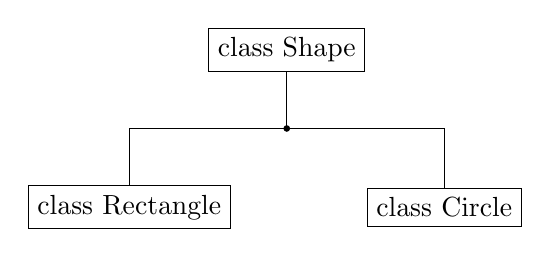
\begin{tikzpicture}
    \node[draw] (shape) at (0,2) {class Shape};
    \node[draw] (rect) at (-2,0) {class Rectangle};
    \node[draw] (circle) at (2,0) {class Circle};
    \draw (shape.south) |- (0,1) -| (rect.north);
    \draw (0,1) -| (node cs:name=circle,anchor=north);
%    \draw (0,1) -| (circle.north);
    \fill (0,1) circle [radius=1.2pt];
\end{tikzpicture}

% 2)角度
% 显式格式: (node cs:name=<name>,angle=<angle>)
%   angle - 指定角度(非弧度值)
% 隐式格式: (<name>.<angle>)


% 相关参数
% 1.shape - 指定背景形状(section 71). 可选列表: 
%   1)circle - 圆
%   2)rectangle - 矩形. 默认形状
%   下列需要使用shapes.geometric
%   3)ellipse - 椭圆
%   4)trapezium - 梯形. 配合选项如下:
%     trapezium left angle - 梯形左下角度数. 默认为60
%     trapezium right angle - 梯形右下角度数,默认为60
%     trapezium angle - 梯形左下角和右下角度数
%   5)semicircle - 半圆
%   6)regular polygon - 正多边形. 配合选项如下:
%     regular polygon sides - 正多边形的边数
%   7)start - 多角星. 配合选项如下:
%     start points - 多角星的角数. 默认为5
%     star point height - 圆半径的差距
%     star point ratio - 圆半径之比, 大圆/小圆. 当小圆半径为大圆半径的0.382时,五角星标准
%   8)isosceles triangle - 等腰三角形. 配合选项如下:
%     isosceles triangle apex angle - 顶角度数. 默认30
%   9)kite - 风筝. 配合选项如下:
%     kite upper vertex angel - 顶角度数. 默认120
%     kite lower vertex angle - 底角度数. 默认60
%     kite vertex angle - 顶角和底角度数
%   10)dart - 镖形. 配合选项如下:
%     dart tip angle - 顶部角. 默认45
%     dart tail angle - 底部角. 默认135
%   11)circular sector - 扇形. 配合选项如下:
%     circular sector angle - 圆心角度数
%   12)cylinder - 圆柱体. 配合选项如下:
%     aspect - 圆柱体底部椭圆的半径比(y_radius/x_radius). 默认为1
%     cylinder uses custom fill - 允许填充圆柱体两端和圆柱
%     cylinder end fill - 两端颜色填充
%     cylinder body fill - 圆柱颜色填充
%   下列需要使用shapes.arrows
%   13)single arrow - 单向箭头. 配合选项如下:
%     single arrow tip angle - 箭头夹角角度
%     single arrow head extend - 箭头尾部和线条的距离
%     single arrow head indent - 箭头尾部缩进尺寸
%   14)double arrow - 双向箭头. 配合选项如下:
%     double arrow tip angle - 箭头夹角角度
%     double arrow head extend - 箭头尾部和线条的距离
%     double arrow head indent - 箭头尾部缩进尺寸
%   下列需要使用shapes.misc
%   15)cross out - 交叉删除线
%   16)strike out - 左下角到右上角的单删除线
%   17)rounded rectangle - 宽为圆弧的矩形. 配合选项如下:
%     rounded rectangle arc length - 宽圆弧对应的圆心角度数, 范围为[90,180]
%     rounded rectangle west arc
%     rounded rectangle left arc - 左侧圆弧类型. 可选类型列表:
%       concave - 内凹圆弧
%       convex - 外凸圆弧
%       none - 无圆弧
%     rounded rectangle east arc
%     rounded rectangle right arc - 右侧圆弧类型. 类型参数左侧圆弧
% 2.draw - 背景边框色
% 3.fill - 背景填充色
% 4.rotate - 旋转node
% 5.shape border rotate - 只旋转边框
% 6.scale - 扩大/缩小node尺寸
% 7.minimum height - 当文字高度和inner sep加起来小于指定值时,进行补足;当文字高度和inner sep加起来大于等于指定值时,不做改变
% 8.minimum width - 类似于minimum height,用于宽度
% 9.minimum size - 同时指定minimum height/width
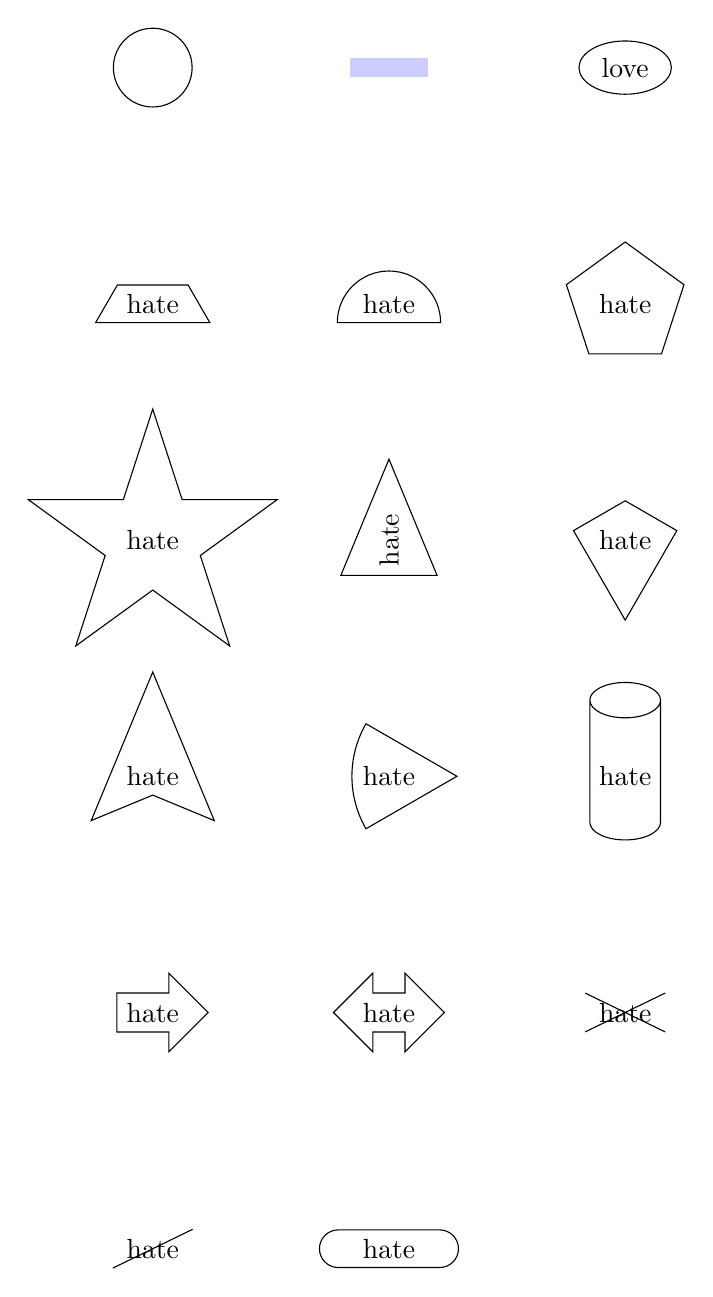
\begin{tikzpicture}
    \node[draw,circle,minimum width=1cm] at (1,0){};
    \node[fill=blue!20,rectangle,minimum width=1cm] at ([xshift=3cm]1,0){};
    \node[draw,ellipse,minimum width=1cm] at ([xshift=6cm]1,0){love};
    \node[draw,trapezium,minimum width=1cm] at ([yshift=-3cm]1,0){hate};
    \node[draw,semicircle,minimum width=1cm] at ([shift={(3cm,-3cm)}]1,0){hate};
    \node[draw,regular polygon,minimum width=1cm] at ([shift={(6cm,-3cm)}]1,0){hate};
    \node[draw,star,star point ratio=1/0.382,minimum width=1cm] at ([shift={(0cm,-6cm)}]1,0){hate};
    \node[draw,rotate=90,isosceles triangle,minimum width=1cm] at ([shift={(3cm,-6cm)}]1,0){hate};
    \node[draw,kite,minimum width=1cm] at ([shift={(6cm,-6cm)}]1,0){hate};
    \node[draw,shape border rotate=90,dart,minimum width=1cm] at ([shift={(0cm,-9cm)}]1,0){hate};
    \node[draw,circular sector,minimum width=1cm] at ([shift={(3cm,-9cm)}]1,0){hate};
    \node[draw,shape border rotate=90,cylinder,aspect=0.5,minimum height=2cm] at ([shift={(6cm,-9cm)}]1,0){hate};
    \node[draw,single arrow,minimum width=1cm] at ([shift={(0cm,-12cm)}]1,0){hate};
    \node[draw,double arrow,minimum width=1cm] at ([shift={(3cm,-12cm)}]1,0){hate};
    \node[draw,cross out,minimum width=1cm] at ([shift={(6cm,-12cm)}]1,0){hate};
    \node[draw,strike out,minimum width=1cm] at ([shift={(0cm,-15cm)}]1,0){hate};
    \node[draw,rounded rectangle,minimum width=2cm] at ([shift={(3cm,-15cm)}]1,0){hate};
\end{tikzpicture}


% 相关参数
% 10.behind path - 配合path时,node在path图层下方
%    in front of path - 配合path时,node在path图层上方
% 11.line width - 边框宽度
% 12.double - 边框使用双线
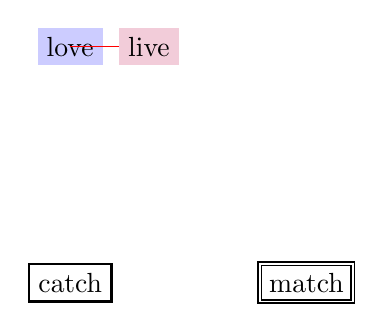
\begin{tikzpicture}[line width=0.6pt]
    \draw[draw=red] (0,0) node[fill=blue!20,behind path]{love} -- (1,0) node[fill=purple!20]{live};
    \node[draw,line width=1pt] at (0,-3){catch};
    \node[draw,double] at (3,-3){match};
\end{tikzpicture}


% 相关参数
% 13.inner sep - 文字与背景边框的距离, 默认为1/3em. 可使用以下参数分别指定x/y轴padding: inner xsep/inner ysep
% 14.outer sep - 背景边框与外部内容的距离, 默认为line width的一半
% 15.color - 边框和文字颜色
% 16.text - 指定文本颜色,必须在color后面指定,不然会被color覆盖
% 17.text opacity - 文本透明度
% 18.text width - 文字所占宽度
% 19.align - 多行文本的对齐方式,文本使用\\主动换行,或根据text width参数值自动换行. 可选参数: 
%   1)left - 左对齐
%   2)flush left - 类似于左对齐,尽量避免分词,比left参数的右侧更错落有致
%   3)right - 右对齐
%   4)flush right - 类似于右对齐,尽量避免分词,比right参数的左侧更错落有致
%   5)center - 居中对齐
%   6)flush center - 类似于居中对齐,尽量避免分词,比center参数的两侧侧更错落有致
%   7)justify - 自动调整单词间隔,使两侧对齐
%   8)none - 不进行对齐
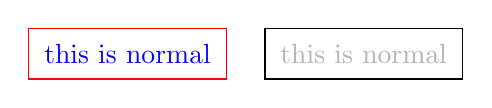
\begin{tikzpicture}[line width=0.6pt]
    \node[draw,inner sep=2mm,color=red,text=blue] at (0,0){this is normal};
    \node[draw,inner sep=2mm,text opacity=0.3] at (3,0){this is normal};
\end{tikzpicture}


% 相关参数
% 20.below - node内容相对于坐标的位置. 可用参数列表如下:
%   1)above - node内容位于坐标上方
%   2)below - node内容位于坐标下方
%   3)left - node内容位于坐标左方
%   4)right - node内容位于坐标右方
%   5)above left - node内容位于坐标左上方
%   6)above right - node内容位于坐标右上方
%   7)below left - node内容位于坐标左下方
%   8)below right - node内容位于坐标右下方
%   9)centered - node内容位于坐标位置
%   备注: below/above/left/right可指定距离值;above left/above right/below left/below right也可指定距离值,并且可以使用<dimension_ver> and <dimension_hori>分别指定垂直距离和水平距离,但需要使用positioning库
% 21.pos - node在路径上(前一个坐标到当前坐标)的位置. 如: 0.5代表路径中点. 也可以使用如下参数:
%   1)at start - 类似于pos=0
%   2)very near start - 类似于pos=0.125
%   3)near start - 类似于pos=0.25
%   4)midway - 类似于pos=0.5
%   5)near end - 类似于pos=0.75
%   6)very near end - 类似于0.875
%   7)at end - 类似于pos=1
\begin{tikzpicture}[line width=0.6pt]
    \node[above] at (0,0){above};
    \node[below] at (0,0){above};
    \node[below left] at (3,0){this is normal};
    \node[above right=10pt and 2pt] at (3,0){this is normal};
    \fill (0,0) circle [radius=1pt];
    \fill (3,0) circle [radius=1pt];
    \draw (0,-3) -- (3,-3) node[pos=0.33,above]{1/3};
\end{tikzpicture}


% 相关参数
%   22.transform shape - 将外部的图形变化操作引入当前node

% update 2025-04-16




% 在坐标点附近添加注释文字
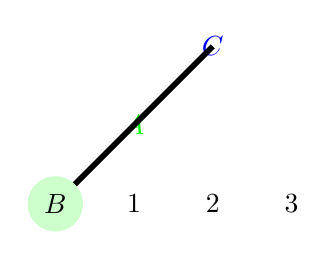
\begin{tikzpicture}

    %   13)shape aspect - 宽度与高度的比率
    %   21)fit - 当前node的尺寸,可以容纳其他node,需要使用fit库. 格式: fit=(A)(B)(B)
    %   25)auto - node相对于路径的位置. 可选列表: left/right
    %   26)swap - 相对于全局auto,当前环境内取auto的相反值
    %   27)sloped - 旋转文字,使文字顺着曲线的方向
    %   28)label - 在node处额外添加其他node. 格式: [<options>]<angle>:<text>. angle可选列表:
    %     [1]above/below/right/left/above left/above right/below left/below right
    %     [2]center - label node与主node的中心重合
    %     [3]角度值 - label的angle会偏向于45度的整数倍,无法精确定位角度
    %   29)pin - 类似于label,在主node与从node间添加连线
    \path node foreach \x in {1,2,3} at (\x,0) {\x};
    \path node (A) [color=green] at (1,1) {$A$};
    \draw[line width=2pt] (0,0) node[fill=green!20,shape=circle]{$B$} -- (2,2) node[behind path,color=blue]{$C$};
\end{tikzpicture}\\\vspace{1cm}

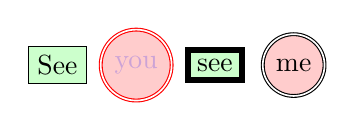
\begin{tikzpicture}
    % 配置所有node的属性
    [every node/.style={fill=green!20,draw},
    % 配置圆形背景node的属性
    every circle node/.style={fill=red!20,double}]
    \path node (A) at (0,0) {See};
    \path node[circle,color=red,text=blue,text opacity=0.2] (B) at (1,0) {you};
    \path node[line width=2pt] (C) at (2,0) {see};
    \path node[circle] (D) at (3,0) {me};
\end{tikzpicture}\\\vspace{1cm}

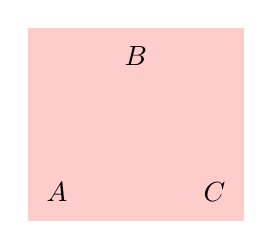
\begin{tikzpicture}
    % fit
    \path node (A) at (0,0) {$A$};
    \path node (B) at (1,1.732) {$B$};
    \path node (C) at (2,0) {$C$};
    \begin{scope}[on background layer]
      \path node[fill=red!20,shape=rectangle,fit=(A)(B)(C)] {}; 
    \end{scope}
\end{tikzpicture}\\\vspace{1cm}

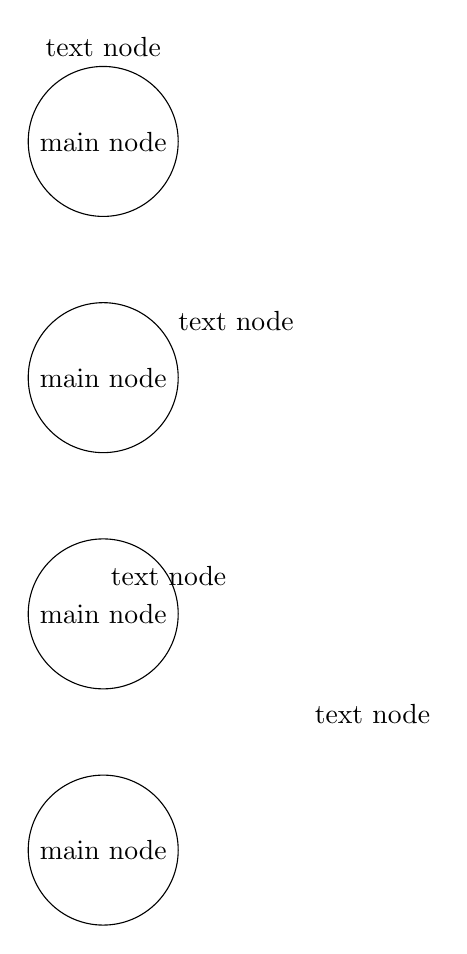
\begin{tikzpicture}
    % 其他node - label
    \path node[circle,draw,label=text node] (A) at (0,0) {main node};
    \path node[circle,draw,label=30:text node] (B) at (0,-3) {main node};
    \path node[circle,draw,label={[centered]30:text node}] (C) at (0,-6) {main node};
    \path node[circle,draw,label={[label distance=2cm]30:text node}] (D) at (0,-9) {main node};
\end{tikzpicture}
\end{document}
